\documentclass[12pt, twoside]{article}
\usepackage[francais]{babel}
\usepackage[T1]{fontenc}
\usepackage[latin1]{inputenc}
\usepackage[left=7mm, right=7mm, top=7mm, bottom=7mm]{geometry}
\usepackage{float}
\usepackage{graphicx}
\usepackage{array}
\usepackage{multirow}
\usepackage{amsmath,amssymb,mathrsfs}
\usepackage{soul}
\usepackage{textcomp}
\usepackage{eurosym}
 \usepackage{variations}
\usepackage{tabvar}


\pagestyle{empty}

\begin{document}


\section*{\center{Devoir maison 5}}


\bigskip





\fbox{

\begin{minipage}{18cm}
\textit{Devoir � rendre sur feuille grand format petits
carreaux pour le \textbf{lundi 8 mars 2010}.}
\end{minipage}
}

\enskip


 \textit{Remarque: La pr�sentation et la r�daction seront pris en compte. }


\enskip


\subsection*{Exercice 1}

\begin{enumerate}
  \item Construire un parall�logramme MATH  de centre S. Placer le point O
  milieu du segment [MA].
  \item Justifier que les droites (OS) et (MH) sont parall�les.
\end{enumerate}


\subsection*{Exercice 2}

\begin{center}
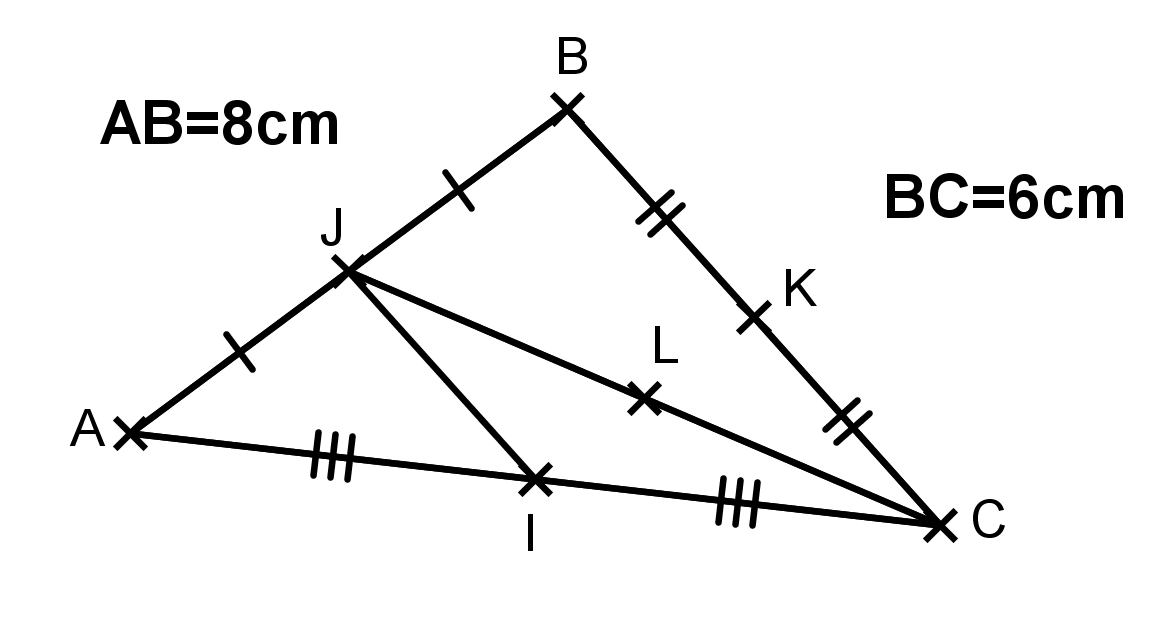
\includegraphics[width=7cm]{images/calcul.png}
\end{center}


\begin{enumerate}
  \item Calculer IJ. Justifier votre r�ponse.
  \item Calculer LK. Justifier votre r�ponse.
\end{enumerate}






 


\subsection*{Exercice 3}

Soit un triangle ABC rectangle en B. Le point I est le milieu de l'hypot�nuse.
La perpendiculaire � (BC) passant par I coupe (BC) en H.
\begin{enumerate}
  \item Faire une figure.
  \item Montrer que les droites (AB) et (HI) sont parall�les.
  \item Le point H est-il le milieu du segment [BC]? Justifier votre r�ponse.
  (vous pouvez r�pondre � cette question en admettant la question 2.)
\end{enumerate}




\subsection*{Exercice 4}


\begin{center}
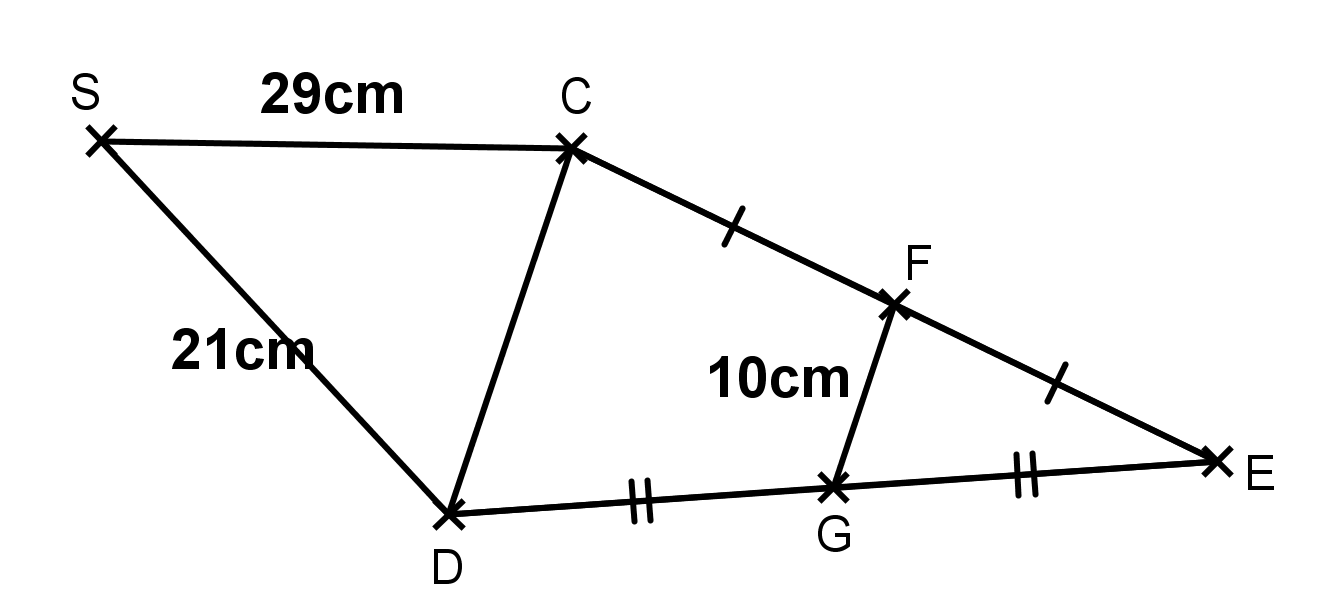
\includegraphics[width=8cm]{images/pb.png}
\end{center}

\begin{enumerate}

\item Calculer DC. Justifier votre r�ponse.
\item Les droites (DS) et (DC) sont-elles prependiculaires? Justifier votre
r�ponse.
\end{enumerate}



\end{document}
